\section{Geodesic Regression}

  In regression, note that we are finding a function $f: \mathcal{X} \to \mathcal{Y}$. In usual linear regression, both $\mathcal{X}, \mathcal{Y}$ are Euclidean space. However, there are cases where it may not be realistic that one or more of them should be modeled as a vector space. Rather, they may be part of a lower-dimensional manifold. For instance, if we want to use linear regression to predict the top $k$ principal components of a dataset, they must be orthogonal, i.e. must be in a \textit{Stiefl manifold}. 

  There are way to model this. For instance, we could have a projection operator that maps from $\mathbb{R}^m \to \mathcal{Y}$. This has its issues too, for one not being very efficient since perhaps the dimension of $\mathcal{Y}$ may be much less than $m$. Therefore, it might be better to directly regress onto a manifold. There were many attempts at this, but the first model to generalize OLS to manifolds was created by Fletcher in 2011 \cite{2011fletcher} and expanded shortly in \cite{2012fletcher}. 

  We start with the case where there is one covariate (i.e. $\mathcal{X} = \mathbb{R}$) and $\mathcal{Y} = (M, d)$ is a smooth Riemannian manifold with a metric. Recall that for a smooth manifold $M$, for any $p \in M$ and $v \in T_p M$, the tangent space at $p$, there is a unique geodesic curve $\gamma: [0, 1] \to M$ satisfying $\gamma(0) = p$, $\gamma^\prime (0) = v$. This geodesic is guaranteed to exist locally, and with this,we can define the exponential map at $p$ in the direction of $v$ as 
  \begin{equation}
    \exp_p (v) = \exp(p, v) = \gamma(1)
  \end{equation}
  In other words, the exponential map takes a position and velocity as input and returns the point at time 1 along the geodesic with these initial conditions. With this motivation, we use slightly different notation than regular linear regression, referring $p$ as the bias and $v$ as the coefficient. 

  \begin{definition}[Geodesic Regression] 
    The \textbf{geodesic regression} model is a probabilistic model that predicts the conditional distribution of $y \in (M, d)$ given $x \in \mathbb{R}$ as 
    \begin{equation}
      y = \exp(\exp(p, vx), \epsilon)
    \end{equation} 
    where the parameters are $\theta = \{p, v\}$, and $\epsilon$ is a random variable defined over the tangent space at $\exp(p, vx)$. 
  \end{definition} 

  Note that if we set $\mathcal{Y} = \mathbb{R}^m$, then we get the ordinary linear regression model back. 

  \begin{definition}[Least Squares Geodesic Regression]
    The least squares geodesic regression aims to minimize the MSE loss 
    \begin{equation}
      L(\theta, (x, y)) = L(p, v, x, y) = d(\exp(p, vx), y)^2
    \end{equation}
  \end{definition}

  \begin{lemma}[Risk]
    The risk is 
    \begin{equation}
      R(f) = \mathbb{E}_{x, y} \left[ d(\exp(p, vx), y)^2 \right]
    \end{equation} 
    and the empirical risk for a dataset $\mathcal{D} = \{(x^{(i)}, y^{(i)})\}_{i=1}^n$ is 
    \begin{equation}
      \hat{R}(f) = \frac{1}{n} \sum_{i=1}^n d(\exp(p, v x^{(i)}), y^{(i)})^2
    \end{equation}
  \end{lemma}

  Unfortunately, minimizing this does not yield an analytic solution. 

  \begin{example}[Code Walkthrough]
    Let us fit a line onto this. We first define our manifold class with the matrix exponential and logarithm methods. 

    \begin{lstlisting}
      class S2:
        @staticmethod
        def exp(p, v):
          v_norm = np.linalg.norm(v)
          if v_norm < 1e-8:
            return p
          return np.cos(v_norm) * p + np.sin(v_norm) * v / v_norm
        
        @staticmethod
        def log(p, q):
          cos_dist = np.clip(np.dot(p, q), -1, 1)
          if np.abs(cos_dist - 1) < 1e-8:
            return np.zeros_like(p)
          
          theta = np.arccos(cos_dist)
          sin_theta = np.sin(theta)
          
          if sin_theta < 1e-8:
            return np.zeros_like(p)
          
          return theta * (q - cos_dist * p) / sin_theta
        
        @staticmethod
        def distance(p, q):
          cos_dist = np.clip(np.dot(p, q), -1, 1)
          return np.arccos(cos_dist)
        
        @staticmethod
        def project_to_tangent(p, v):
          return v - np.dot(v, p) * p
        
        @staticmethod
        def normalize(x):
          return x / np.linalg.norm(x)
    \end{lstlisting}

    Next, we define our data generation process. 

    \begin{lstlisting}
      def generate_sample_data(n_samples=50, noise_level=0.1):
        X = np.random.uniform(-2, 2, n_samples)
        
        p_true = S2.normalize(np.array([1, 0, 0]))
        v_true = S2.normalize(np.array([0, 1, 0.2]))
        v_true = S2.project_to_tangent(p_true, v_true) * 0.5
        
        Y = []
        for x in X:
          y_clean = S2.exp(p_true, v_true * x)
          
          noise = np.random.normal(0, noise_level, 3)
          noise = S2.project_to_tangent(y_clean, noise)
          y_noisy = S2.exp(y_clean, noise)
          y_noisy = S2.normalize(y_noisy)
          
          Y.append(y_noisy)
        
        return X, np.array(Y), p_true, v_true
    \end{lstlisting}

    Finally, we define our regression model and optimize the loss with BFGS (SGD doesn't work very well here). 

    \begin{lstlisting}
      class GeodesicRegression:
        def __init__(self):
          self.p = None
          self.v = None
        
        def _geodesic_point(self, p, v, x):
          return S2.exp(p, v * x)
        
        def _objective(self, params, X, Y):
          p_flat = params[:3]
          v_flat = params[3:6]
          
          p_flat = S2.normalize(p_flat)
          v_flat = S2.project_to_tangent(p_flat, v_flat)
          
          total_loss = 0.0
          for i in range(len(X)):
            pred = self._geodesic_point(p_flat, v_flat, X[i])
            loss = S2.distance(pred, Y[i])**2
            total_loss += loss
          
          return total_loss / len(X)
        
        def fit(self, X, Y, p_init=None, v_init=None, method='BFGS'):
          X = np.array(X)
          Y = np.array(Y)
          
          if p_init is None:
            p_init = S2.normalize(np.array([1, 0, 0]))
          if v_init is None:
            v_init = np.array([0, 0.1, 0])
          
          v_init = S2.project_to_tangent(p_init, v_init)
          
          initial_params = np.concatenate([p_init, v_init])
          
          result = minimize(
            self._objective,
            initial_params,
            args=(X, Y),
            method=method,
            options={'disp': False}
          )
          
          if result.success:
            self.p = S2.normalize(result.x[:3])
            self.v = S2.project_to_tangent(self.p, result.x[3:6])
            return result
          else:
            raise RuntimeError(f"Optimization failed: {result.message}")
        
        def predict(self, X):
          X = np.array(X)
          predictions = []
          
          for x in X:
            pred = self._geodesic_point(self.p, self.v, x)
            predictions.append(pred)
          
          return np.array(predictions)
        
        def score(self, X, Y):
          predictions = self.predict(X)
          total_loss = 0.0
          
          for i in range(len(Y)):
            loss = S2.distance(predictions[i], Y[i])**2
            total_loss += loss
          
          return total_loss / len(Y)

      X_train, Y_train, p_true, v_true = generate_sample_data(n_samples=30)
      model = GeodesicRegression()
      result = model.fit(X_train, Y_train)
    \end{lstlisting}
    
    This gives the following, which is a good estimate of the original parameters. 

    \begin{equation}
      \hat{p} = \begin{pmatrix} 0.99993911 \\ -0.01038634 \\ -0.00372747 \end{pmatrix} \approx \begin{pmatrix} 1 \\ 0 \\ 0 \end{pmatrix} = p_{\mathrm{true}}, \qquad 
      \hat{v} = \begin{pmatrix} 0.00530609 \\ 0.48332324 \\ 0.07667702 \end{pmatrix} \approx \begin{pmatrix} 0 \\ 0.49029034 \\ 0.09805807 \end{pmatrix} = v_{\mathrm{true}}
    \end{equation}

    The following figure also visualizes this. 

    \begin{figure}[H]
      \centering  
      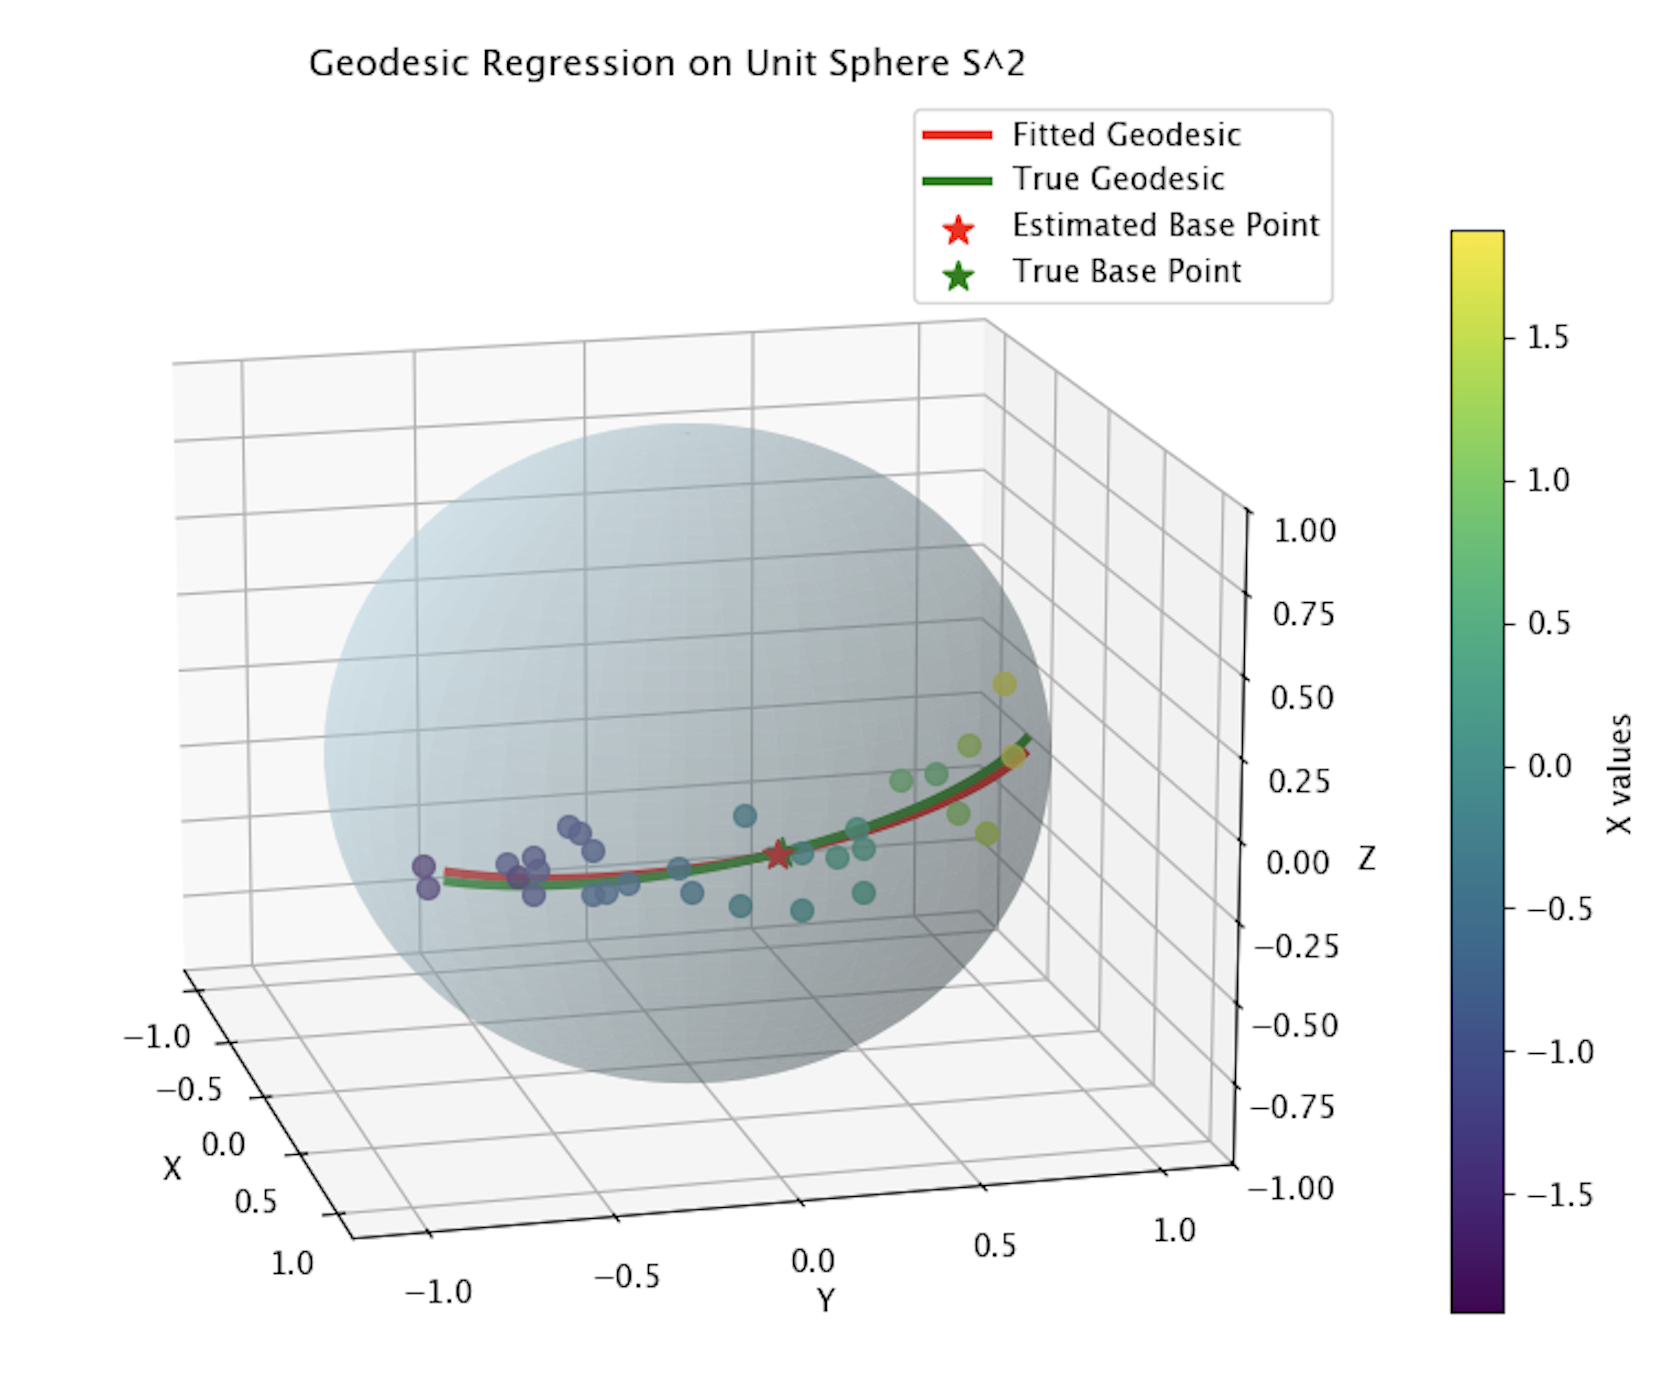
\includegraphics[scale=0.4]{img/geodesic_sphere.png}
      \caption{} 
    \end{figure}
  \end{example}

\subsection{Multiple Geodesic Regression} 

  Note that this was a model for a path in some manifold, and naturally we would like to extend this to have multiple covariates. Kim in 2014 did exactly that, and provided a framework for multivariate general linear models in \cite{2014kim}.  

  \begin{definition}[Multiple Geodesic Regression] 
    The \textbf{multiple geodesic regression} model is a probabilistic model that predicts the conditional distribution of $y \in (M, d)$ given $x \in \mathbb{R}$ as 
    \begin{equation}
      y = \exp \bigg( \exp \Big( p, \sum_{i=1}^d x_j v_j \Big), \epsilon \bigg) = \exp \big( \exp (p, V x)\big)
    \end{equation} 
    where the parameters are $\theta = \{p \in \mathbb{R}^m, V \in \mathbb{R}^{m \times d}\}$, and $\epsilon$ is a random variable defined over the tangent space at $\exp(p, Vx)$. 
  \end{definition} 

  \begin{definition}[Least Squares Geodesic Regression]
    The least squares geodesic regression aims to minimize the MSE loss 
    \begin{equation}
      L(\theta, (x, y)) = L(p, v, x, y) = d(\exp(p, Vx), y)^2
    \end{equation}
  \end{definition} 

  \begin{example}[Code Walkthrough]
    We demonstrate this by conducting geodesic regression on a dataset of 50 samples $(x \in \mathbb{R}^2, y \in S^2)$. We start by generating a 2-dimensional toy dataset according to our model. 

    \begin{lstlisting}
      def generate_sample_data(n_samples=50, n_features=2, noise_level=0.1):
        X = np.random.uniform(-1, 1, (n_samples, n_features))
        
        p_true = S2.normalize(np.array([1, 0, 0]))
        V_true = np.array([[0, 0.3], [0.5, -0.2], [0.2, 0.4]])
        
        for i in range(n_features):
          V_true[:, i] = S2.project_to_tangent(p_true, V_true[:, i])
        
        Y = []
        for x in X:
          tangent_vec = V_true @ x
          y_clean = S2.exp(p_true, tangent_vec)
          
          noise = np.random.normal(0, noise_level, 3)
          noise = S2.project_to_tangent(y_clean, noise)
          y_noisy = S2.exp(y_clean, noise)
          y_noisy = S2.normalize(y_noisy)
          
          Y.append(y_noisy)
        
        return X, np.array(Y), p_true, V_true
    \end{lstlisting}

    \begin{lstlisting}
      class MultipleGeodesicRegression:
        def __init__(self, n_features):
          self.n_features = n_features
          self.p = None
          self.V = None
        
        def _geodesic_point(self, p, V, x):
          tangent_vec = V @ x
          return S2.exp(p, tangent_vec)
        
        def _objective(self, params, X, Y):
          p_flat = params[:3]
          V_flat = params[3:].reshape(3, self.n_features)
          
          p_flat = S2.normalize(p_flat)
          
          for i in range(self.n_features):
            V_flat[:, i] = S2.project_to_tangent(p_flat, V_flat[:, i])
          
          total_loss = 0.0
          for i in range(len(X)):
            pred = self._geodesic_point(p_flat, V_flat, X[i])
            loss = S2.distance(pred, Y[i])**2
            total_loss += loss
          
          return total_loss / len(X)
        
        def fit(self, X, Y, p_init=None, V_init=None, method='BFGS'):
          X = np.array(X)
          Y = np.array(Y)
          
          if p_init is None:
            p_init = S2.normalize(np.array([1, 0, 0]))
          if V_init is None:
            V_init = np.random.normal(0, 0.1, (3, self.n_features))
          
          for i in range(self.n_features):
            V_init[:, i] = S2.project_to_tangent(p_init, V_init[:, i])
          
          initial_params = np.concatenate([p_init, V_init.flatten()])
          
          result = minimize(
            self._objective,
            initial_params,
            args=(X, Y),
            method=method,
            options={'disp': False}
          )
          
          if result.success:
            self.p = S2.normalize(result.x[:3])
            self.V = result.x[3:].reshape(3, self.n_features)
            
            for i in range(self.n_features):
              self.V[:, i] = S2.project_to_tangent(self.p, self.V[:, i])
            
            return result
          else:
            raise RuntimeError(f"Optimization failed: {result.message}")
        
        def predict(self, X):
          X = np.array(X)
          predictions = []
          
          for x in X:
            pred = self._geodesic_point(self.p, self.V, x)
            predictions.append(pred)
          
          return np.array(predictions)
        
        def score(self, X, Y):
          predictions = self.predict(X)
          total_loss = 0.0
          
          for i in range(len(Y)):
            loss = S2.distance(predictions[i], Y[i])**2
            total_loss += loss
          
          return total_loss / len(Y)
    \end{lstlisting}

    The results show that it is a good estimate. Both the initial point $\hat{p}$ and the matrix $\hat{V}$ are good estimators. 
    \begin{equation}
      \hat{p} = \begin{pmatrix} 0.99984466 \\ 0.01430395 \\ 0.01029851 \end{pmatrix} \approx \begin{pmatrix} 1 \\ 0 \\ 0 \end{pmatrix} = p, \qquad \hat{V} =  \begin{pmatrix}
        -0.00905151 & -0.00171887 \\
        0.48494844 & -0.18346139 \\
        0.20521662 & 0.42169444
      \end{pmatrix}
      \approx \begin{pmatrix} 0 & 0 \\ 0.5 & -0.2 \\ 0.2 & 0.4  \end{pmatrix} = V
    \end{equation}

    \begin{figure}[H]
      \centering 
      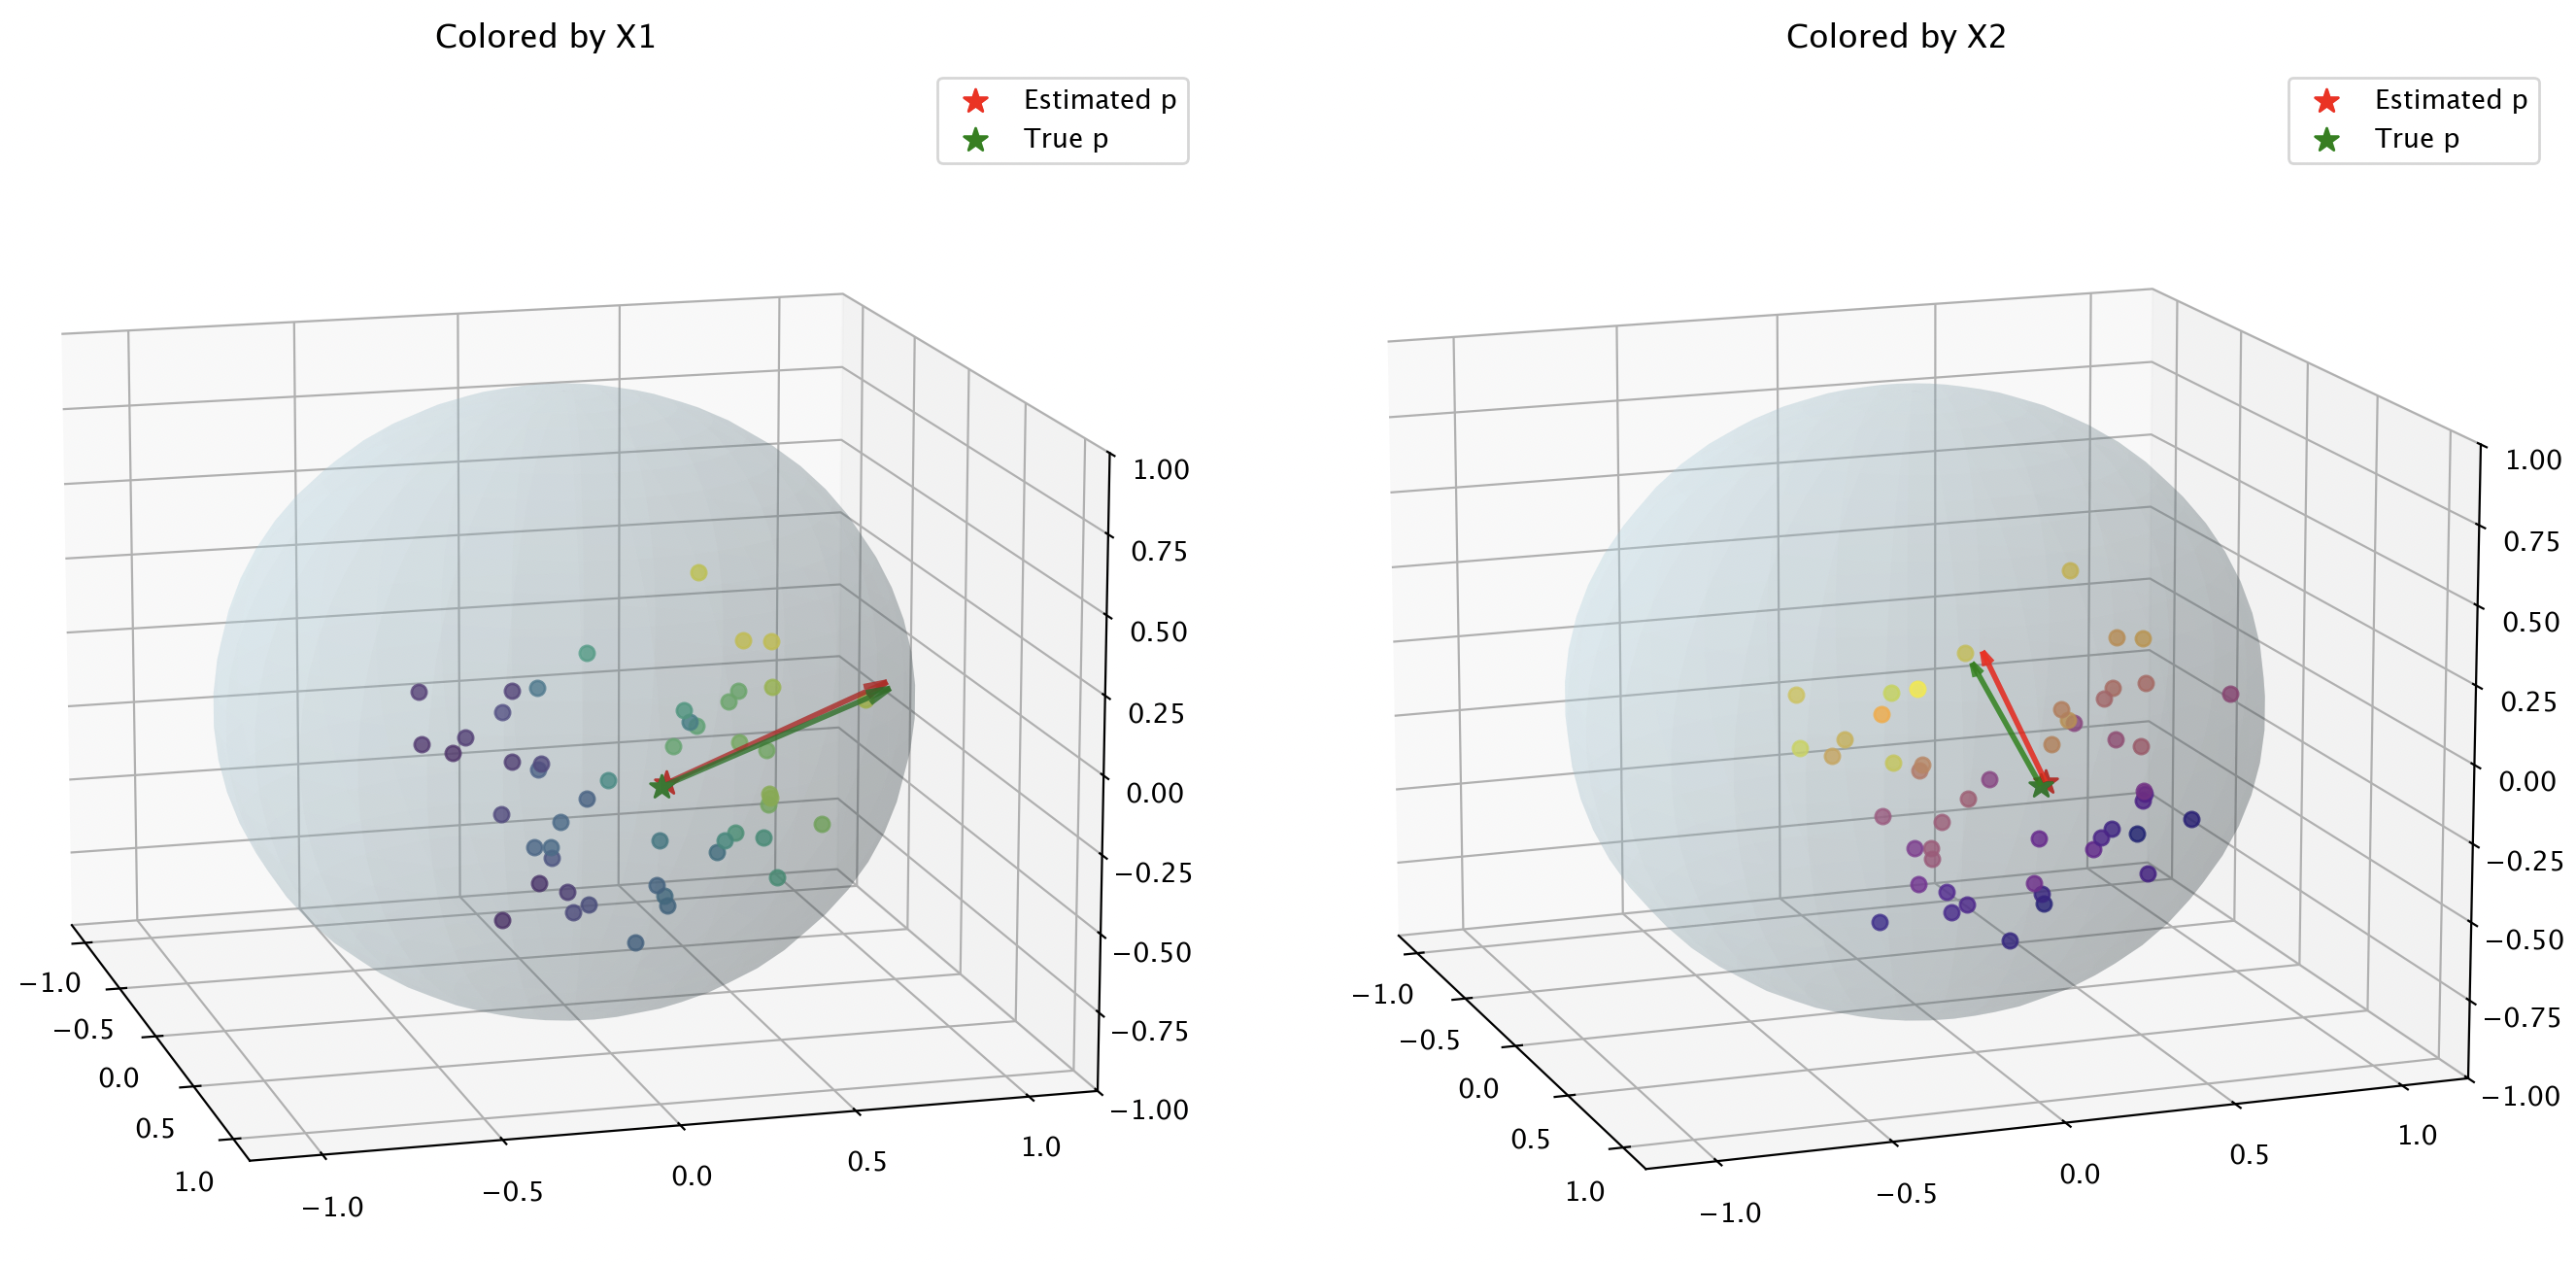
\includegraphics[scale=0.32]{img/multi_geodesic_est.png}
      \caption{The estimated values of the first column of $V$ (left) and the second column of $V$ (right) are good approximations of the true. Note that they point in the direction of the gradients.} 
    \end{figure}

    \begin{figure}[H]
      \centering 
      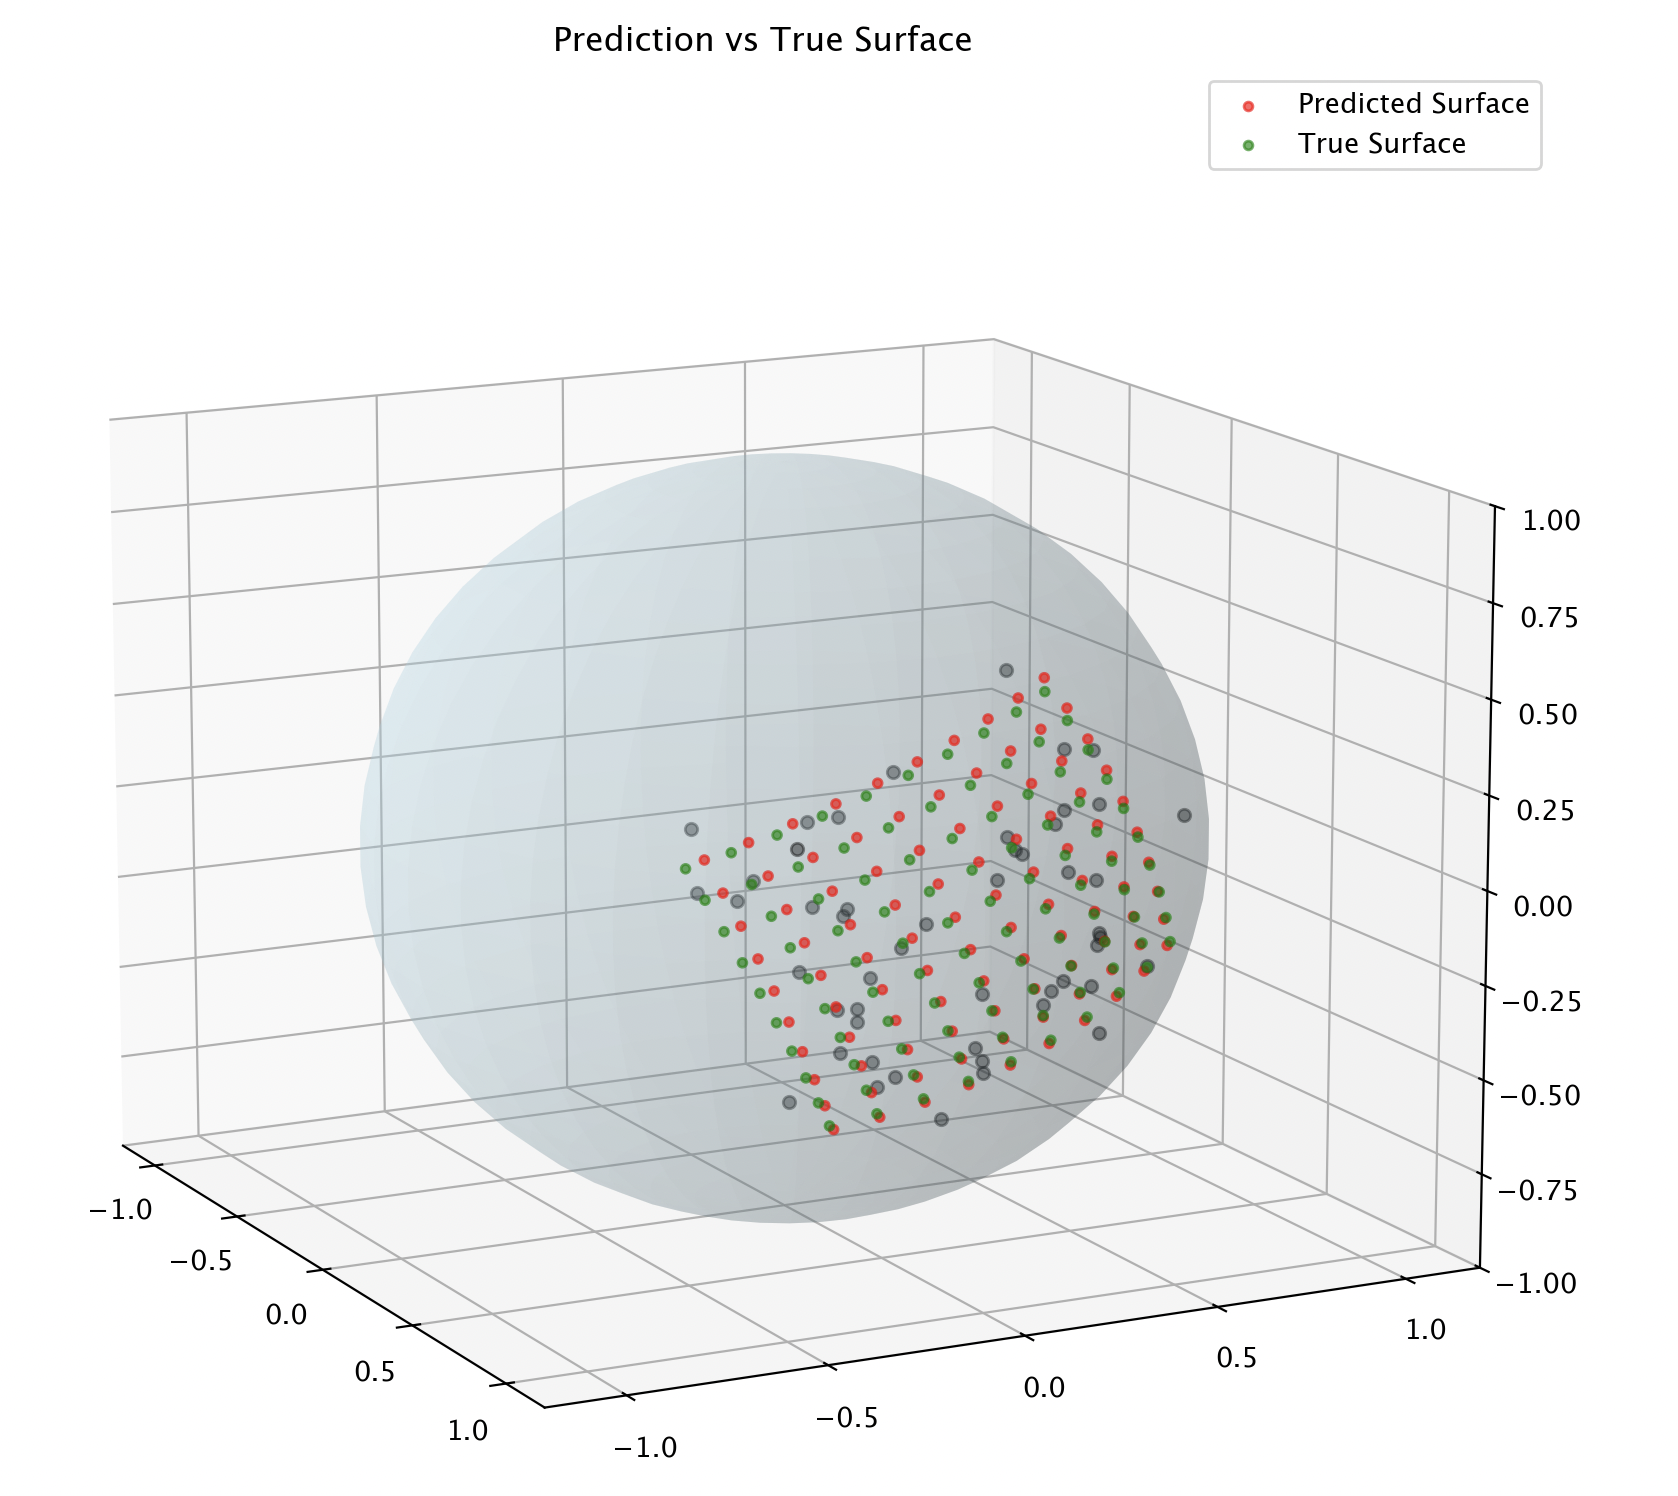
\includegraphics[scale=0.3]{img/multi_geodesic_surface.png}
      \caption{Since we are regressing a 2-dimensional space onto a 2-dimensional manifold, the image of $f$ is trivially $S^2$ except in degenerate cases. However, it is still nice to compare our predicted values $\hat{y} = f(x)$ to the true $y$.} 
    \end{figure}
  \end{example}

\subsection{Robust Geodesic Regression} 
